\documentclass{beamer}
\usepackage{tikz}
\usetheme{Warsaw}  %% Themenwahl

\title{DiDy Application Talk}
\author{Marten Heidemeyer}
\date{\today}

\begin{document}
\maketitle
\frame{\tableofcontents[currentsection]}

\section{About Me}
\begin{frame} %%Eine Folie
  \frametitle{CV} %%Folientitel
  {\renewcommand{\arraystretch}{1.8} 
  \begin{tabular}{ r l }
  Sep. 2009 - Mar. 2013: & \parbox[t]{5cm}{B.Sc. Computing Science,\\Universit{\"a}t zu L{\"u}beck}  \\
  Aug. 2013 - May 2014: & Java Developer, Hamburg S{\"u}d\\
  Sep. 2014 - (expected) Sep. 2016: & \parbox[t]{5cm}{M.Sc. Computing Science,\\Simon Fraser University} \\
  Currently: & \parbox[t]{5cm}{Exchange student,\\Universit{\"a}t Bielefeld}
\end{tabular}}
\end{frame}


\section{My Master Thesis}
\begin{frame} %%Eine Folie
  \frametitle{Drug Target Interaction Prediction} %%Folientitel
  \begin{itemize}
  \item two entities: ligands (drugs) and proteins (targets).
  \item Drug Discovery: find the ligand that binds (only) to the target protein.
  \item off-target binding $\Rightarrow$ side effects
  \item wetlab experiments to verify binding behaviour of ligands are expensive.
  \end{itemize}
\end{frame}

\begin{frame}
\frametitle{Problem Definition}
\begin{itemize}
\item given a sparsely populated matrix of $|D|$ drugs and $|T|$ targets
\item observed values: experimentally verified binding strength of $d_i$ and $t_j$.
\item Goal: predict missing values
\item Benchmark dataset \textit{Metz}: 1421 drugs, 156 targets, \mbox{40\% density}, training data $\in [4, 10] Kd$  
\end{itemize}
\end{frame}

\begin{frame}
\only<1>{
Input
\begin{itemize}
\item Train/Test data:
\end{itemize}
\begin{center}
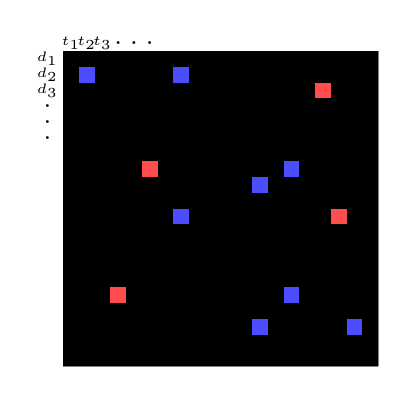
\begin{tikzpicture}[scale=0.2]
\draw[help lines] (0,0) grid (20,20);
\fill [black] (0,0) rectangle (20,20);
\fill [red!70] (3,4) rectangle (4,5);
\fill [red!70] (5,12) rectangle (6,13);
\fill [blue!70] (14,12) rectangle (15,13);
\fill [red!70] (12,2) rectangle (13,3);
\fill [blue!70] (12,2) rectangle (13,3);
\fill [blue!70] (12,11) rectangle (13,12);
\fill [blue!70] (7,9) rectangle (8,10);
\fill [red!70] (17,9) rectangle (18,10);
\fill [blue!70] (7,18) rectangle (8,19);
\fill [blue!70] (1,18) rectangle (2,19);
\fill [blue!70] (18,2) rectangle (19,3);
\fill [blue!70] (14,4) rectangle (15,5);
\fill [red!70] (16,17) rectangle (17,18);
\node at(-1,19.5) {\tiny $d_1$};
\node at(-1,18.5) {\tiny $d_2$};
\node at(-1,17.5) {\tiny $d_3$};
\node at(-1,16.5) {$.$};
\node at(-1,15.5) {$.$};
\node at(-1,14.5) {$.$};

\node at(0.5,20.5) {\tiny $t_1$};
\node at(1.5,20.5) {\tiny $t_2$};
\node at(2.5,20.5) {\tiny $t_3$};

\node at(3.5,20.5) {$.$};
\node at(4.5,20.5) {$.$};
\node at(5.5,20.5) {$.$};
\end{tikzpicture}
\end{center}
\begin{itemize}
\item Similarity matrices for drugs and targets (Assumption: similar drugs bind to similar targets)
\end{itemize}}
\only<2>{
Input
\begin{itemize}
\item Train/Test data:
\end{itemize}
\begin{center}
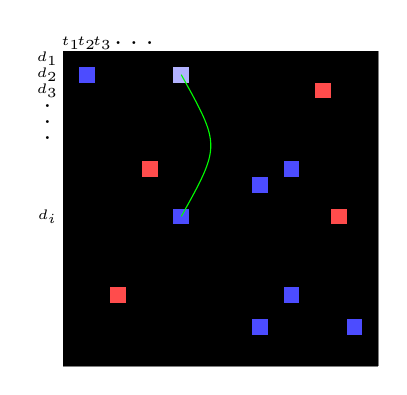
\begin{tikzpicture}[scale=0.2]
\draw[help lines] (0,0) grid (20,20);
\fill [black] (0,0) rectangle (20,20);
\fill [red!70] (3,4) rectangle (4,5);
\fill [red!70] (5,12) rectangle (6,13);
\fill [blue!70] (14,12) rectangle (15,13);
\fill [red!70] (12,2) rectangle (13,3);
\fill [blue!70] (12,2) rectangle (13,3);
\fill [blue!70] (12,11) rectangle (13,12);
\fill [blue!70] (7,9) rectangle (8,10);
\fill [red!70] (17,9) rectangle (18,10);
\fill [blue!30] (7,18) rectangle (8,19);
\fill [blue!70] (1,18) rectangle (2,19);
\fill [blue!70] (18,2) rectangle (19,3);
\fill [blue!70] (14,4) rectangle (15,5);
\fill [red!70] (16,17) rectangle (17,18);
\node at(-1,19.5) {\tiny $d_1$};
\node at(-1,18.5) {\tiny $d_2$};
\node at(-1,17.5) {\tiny $d_3$};
\node at(-1,9.5) {\tiny $d_i$};
\node at(-1,16.5) {$.$};
\node at(-1,15.5) {$.$};
\node at(-1,14.5) {$.$};

\node at(0.5,20.5) {\tiny $t_1$};
\node at(1.5,20.5) {\tiny $t_2$};
\node at(2.5,20.5) {\tiny $t_3$};

\node at(3.5,20.5) {$.$};
\node at(4.5,20.5) {$.$};
\node at(5.5,20.5) {$.$};

\draw [color=green] (7.5,9.5) .. controls (10,14) .. (7.5,18.5);
\end{tikzpicture}
\end{center}
\begin{itemize}
\item Similarity matrices for drugs and targets (Assumption: similar drugs bind to similar targets)
\end{itemize}
}
\only<3>{
Input
\begin{itemize}
\item Train/Test data:
\end{itemize}
\begin{center}
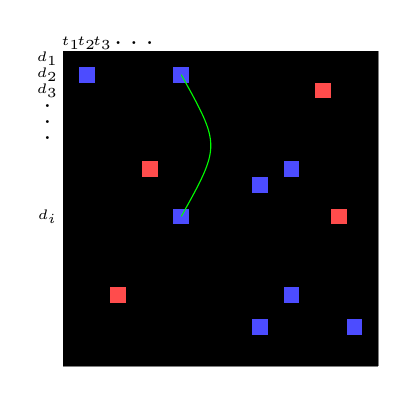
\begin{tikzpicture}[scale=0.2]
\draw[help lines] (0,0) grid (20,20);
\fill [black] (0,0) rectangle (20,20);
\fill [red!70] (3,4) rectangle (4,5);
\fill [red!70] (5,12) rectangle (6,13);
\fill [blue!70] (14,12) rectangle (15,13);
\fill [red!70] (12,2) rectangle (13,3);
\fill [blue!70] (12,2) rectangle (13,3);
\fill [blue!70] (12,11) rectangle (13,12);
\fill [blue!70] (7,9) rectangle (8,10);
\fill [red!70] (17,9) rectangle (18,10);
\fill [blue!70] (7,18) rectangle (8,19);
\fill [blue!70] (1,18) rectangle (2,19);
\fill [blue!70] (18,2) rectangle (19,3);
\fill [blue!70] (14,4) rectangle (15,5);
\fill [red!70] (16,17) rectangle (17,18);
\node at(-1,19.5) {\tiny $d_1$};
\node at(-1,18.5) {\tiny $d_2$};
\node at(-1,17.5) {\tiny $d_3$};
\node at(-1,9.5) {\tiny $d_i$};
\node at(-1,16.5) {$.$};
\node at(-1,15.5) {$.$};
\node at(-1,14.5) {$.$};

\node at(0.5,20.5) {\tiny $t_1$};
\node at(1.5,20.5) {\tiny $t_2$};
\node at(2.5,20.5) {\tiny $t_3$};

\node at(3.5,20.5) {$.$};
\node at(4.5,20.5) {$.$};
\node at(5.5,20.5) {$.$};

\draw [color=green] (7.5,9.5) .. controls (10,14) .. (7.5,18.5);
\end{tikzpicture}
\end{center}
\begin{itemize}
\item Similarity matrices for drugs and targets (Assumption: similar drugs bind to similar targets)
\end{itemize}
}
\end{frame}


\begin{frame} %%Eine Folie
  \frametitle{Model} %%Folientitel
  \begin{center}
  	Matrix Factorization + Continuous Conditional Random Fields
  \end{center}
  
  
  \begin{center}
  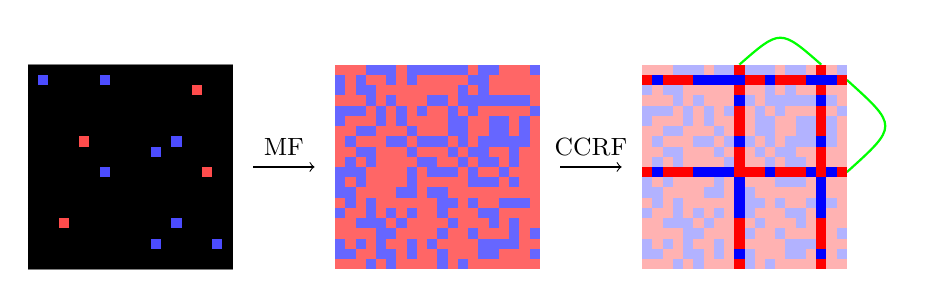
\begin{tikzpicture}[scale=0.13]
  
  \foreach \x in {0,...,19}
  	\foreach \y in {0,...,19}{
   	 \fill [red!60] (\x+30,\y) rectangle (\x+31,\y+1);
   	 \fill [red!30] (\x+60,\y) rectangle (\x+61,\y+1);
   	 }
   	 
   \foreach \x in {0,...,200}{
   	 \pgfmathsetmacro{\Xa}{random(19)}
   	 \pgfmathsetmacro{\Xb}{random(19)}
   	  \fill [blue!60] (\Xa+29,\Xb) rectangle (\Xa+30,\Xb+1);
   	  \fill [blue!60] (33,0) rectangle (34,1);
   	  \fill [blue!60] (35,0) rectangle (36,1);
   	  \fill [blue!60] (40,0) rectangle (41,1);
   	  \fill [blue!60] (42,0) rectangle (43,1);
   	  \fill [blue!60] (49,19) rectangle (50,20);
   	  \fill [blue!60] (49,15) rectangle (50,16);
   	  \fill [blue!60] (49,1) rectangle (50,2);
   	  \fill [blue!60] (49,3) rectangle (50,4);
   	  
   	  \fill [blue!30] (\Xa+59,\Xb) rectangle (\Xa+60,\Xb+1);
   	  \fill [blue!30] (63,0) rectangle (64,1);
   	  \fill [blue!30] (65,0) rectangle (66,1);
   	  \fill [blue!30] (70,0) rectangle (71,1);
   	  \fill [blue!30] (72,0) rectangle (73,1);
   	  \fill [blue!30] (79,19) rectangle (80,20);
   	  \fill [blue!30] (79,15) rectangle (80,16);
   	  \fill [blue!30] (79,1) rectangle (80,2);
   	  \fill [blue!30] (79,3) rectangle (80,4);
   	  }
   	  
   	  \draw [->] (22,10) to (28,10);
   	  
   	  \draw[help lines] (0,0) grid (20,20);
\fill [black] (0,0) rectangle (20,20);
\fill [red!70] (3,4) rectangle (4,5);
\fill [red!70] (5,12) rectangle (6,13);
\fill [blue!70] (14,12) rectangle (15,13);
\fill [red!70] (12,2) rectangle (13,3);
\fill [blue!70] (12,2) rectangle (13,3);
\fill [blue!70] (12,11) rectangle (13,12);
\fill [blue!70] (7,9) rectangle (8,10);
\fill [red!70] (17,9) rectangle (18,10);
\fill [blue!70] (7,18) rectangle (8,19);
\fill [blue!70] (1,18) rectangle (2,19);
\fill [blue!70] (18,2) rectangle (19,3);
\fill [blue!70] (14,4) rectangle (15,5);
\fill [red!70] (16,17) rectangle (17,18);

\draw [->] (52,10) to (58,10);

\draw [color=green, thick] (80,9.5) .. controls (85,14) .. (80,18.5);
\draw [color=green, thick] (69.5,20) .. controls (73.5,23.5) .. (77.5,20);
%\draw [color=green, thick] (62.5,20) .. controls (65.5,23.5) .. (68.5,20);
%\draw [color=green, thick] (80,2.5) .. controls (85,8.5) .. (80,14.5);

\foreach \x in {0,...,19}{
	\fill [red] (\x+60,18) rectangle (\x+61,19);
	\fill [red] (\x+60,9) rectangle (\x+61,10);
	%\fill [red] (\x+60,2) rectangle (\x+61,3);
	%\fill [red] (\x+60,14) rectangle (\x+61,15);
	\fill [red] (69,\x) rectangle (70,\x+1);
	\fill [red] (77,\x) rectangle (78,\x+1);
	%\fill [red] (62,\x) rectangle (63,\x+1);
	%\fill [red] (68,\x) rectangle (69,\x+1);
}
\foreach \x in {0,...,10}{
   	 \pgfmathsetmacro{\Xa}{random(19)}
   	 	\fill [blue] (\Xa+60,18) rectangle (\Xa+61,19);
   	 	\fill [blue] (\Xa+60,9) rectangle (\Xa+61,10);
   	 	
   	 	
   	 	\fill [blue] (69,\Xa) rectangle (70,\Xa+1);
   	 	\fill [blue] (77,\Xa) rectangle (78,\Xa+1);
   	}
   	
   	\node at(55,12){\small CCRF};
   	\node at(25,12){\small MF};
	\end{tikzpicture} 
	
	\end{center}
	
\end{frame}

\begin{frame}
Making predictions for drug $d_i$.
\begin{itemize}
\item learn two parameters:
\begin{itemize}
\item $\alpha$: how much can we trust the prediction of MF ($X$)
\item $\beta$: how much can we interpolate between similar targets (red edges).
\end{itemize}
\end{itemize}
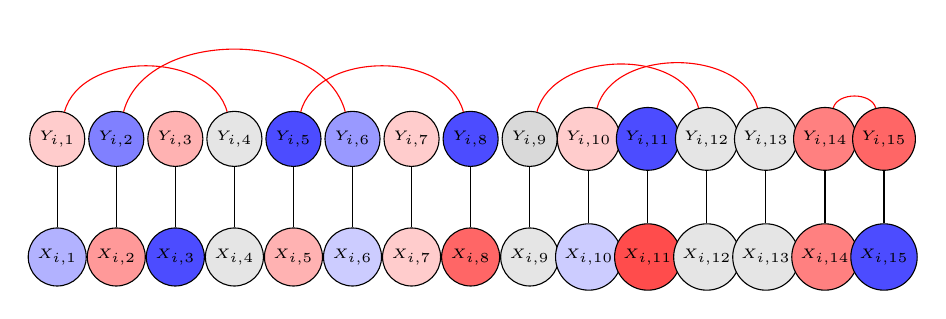
\begin{tikzpicture}[scale=.5]
\tikzstyle{every node} = [draw, shape=circle,minimum size=7mm,inner sep=2pt]
\node [fill = red!20] (a) at (0, 0) {\tiny $Y_{i, 1}$};
\node [fill = blue!50] (b) at (1.5, 0) {\tiny $Y_{i, 2}$};
\node [fill = red!30](c) at (3, 0) {\tiny $Y_{i, 3}$};
\node [fill = gray!20](d) at (4.5, 0) {\tiny $Y_{i, 4}$};
\node [fill = blue!70](e) at (6, 0) {\tiny $Y_{i, 5}$};
\node [fill = blue!40](f) at (7.5, 0) {\tiny $Y_{i, 6}$};
\node [fill = red!20] (g) at (9, 0) {\tiny $Y_{i, 7}$};
\node [fill = blue!70](h) at (10.5, 0) {\tiny $Y_{i, 8}$};
\node [fill = gray!30](i) at (12, 0) {\tiny $Y_{i, 9}$};
\node [fill = red!20](j) at (13.5, 0) {\tiny $Y_{i, 10}$};
\node [fill = blue!70](k) at (15, 0) {\tiny $Y_{i, 11}$};
\node [fill = gray!20](l) at (16.5, 0) {\tiny $Y_{i, 12}$};
\node [fill = gray!20](m) at (18, 0) {\tiny $Y_{i, 13}$};
\node [fill = red!50](n) at (19.5, 0) {\tiny $Y_{i, 14}$};
\node [fill = red!60](o) at (21, 0) {\tiny $Y_{i, 15}$};

\node [fill = blue!30] (ax) at (0, -3) {\tiny $X_{i, 1}$};
\node [fill = red!40](bx) at (1.5, -3) {\tiny $X_{i, 2}$};
\node [fill = blue!70](cx) at (3, -3) {\tiny $X_{i, 3}$};
\node [fill = gray!20](dx) at (4.5, -3) {\tiny $X_{i, 4}$};
\node [fill = red!30](ex) at (6, -3) {\tiny $X_{i, 5}$};
\node [fill = blue!20](fx) at (7.5, -3) {\tiny $X_{i, 6}$};
\node [fill = red!20](gx) at (9, -3) {\tiny $X_{i, 7}$};
\node [fill = red!60](hx) at (10.5, -3) {\tiny $X_{i, 8}$};
\node [fill = gray!20](ix) at (12, -3) {\tiny $X_{i, 9}$};
\node [fill = blue!20](jx) at (13.5, -3) {\tiny $X_{i, 10}$};
\node [fill = red!70](kx) at (15, -3) {\tiny $X_{i, 11}$};
\node [fill = gray!20](lx) at (16.5, -3) {\tiny $X_{i, 12}$};
\node [fill = gray!20](mx) at (18, -3) {\tiny $X_{i, 13}$};
\node [fill = red!50](nx) at (19.5, -3) {\tiny $X_{i, 14}$};
\node [fill = blue!70](ox) at (21, -3) {\tiny $X_{i, 15}$};

\draw [-] (ax) to  [out=90,in=270] (a);
\draw [-] (bx) to  [out=90,in=270] (b);
\draw [-] (cx) to  [out=90,in=270] (c);
\draw [-] (dx) to  [out=90,in=270] (d);
\draw [-] (ex) to  [out=90,in=270] (e);
\draw [-] (fx) to  [out=90,in=270] (f);
\draw [-] (gx) to  [out=90,in=270] (g);
\draw [-] (hx) to  [out=90,in=270] (h);
\draw [-] (ix) to  [out=90,in=270] (i);
\draw [-] (jx) to  [out=90,in=270] (j);
\draw [-] (kx) to  [out=90,in=270] (k);
\draw [-] (lx) to  [out=90,in=270] (l);
\draw [-] (mx) to  [out=90,in=270] (m);
\draw [-] (nx) to  [out=90,in=270] (n);
\draw [-] (ox) to  [out=90,in=270] (o);

\draw [-, draw=red] (a) to  [out=75,in=105] (d);
\draw [-, draw=red] (e) to  [out=75,in=105] (h);
\draw [-, draw=red] (b) to  [out=75,in=105] (f);
\draw [-, draw=red] (j) to  [out=75,in=105] (m);
\draw [-, draw=red] (n) to  [out=75,in=105] (o);
\draw [-, draw=red] (i) to  [out=75,in=105] (l);

\end{tikzpicture}
\end{frame}

\begin{frame}
Example:
\vspace{-2cm}
\begin{center}
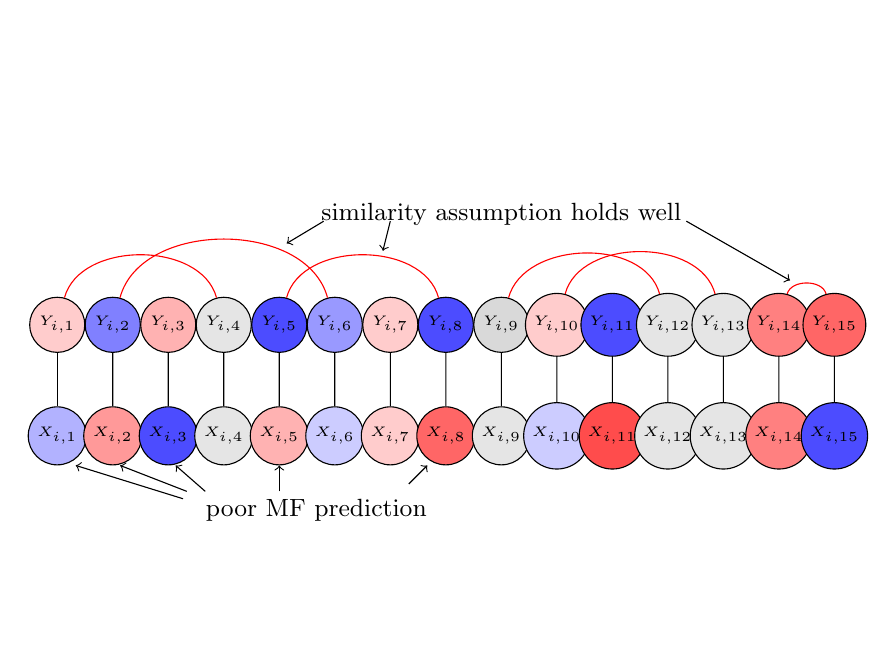
\begin{tikzpicture}[scale=.47]
\tikzstyle{every node} = [draw, shape=circle,minimum size=7mm,inner sep=2pt]
\node [fill = red!20] (a) at (0, 0) {\tiny $Y_{i, 1}$};
\node [fill = blue!50] (b) at (1.5, 0) {\tiny $Y_{i, 2}$};
\node [fill = red!30](c) at (3, 0) {\tiny $Y_{i, 3}$};
\node [fill = gray!20](d) at (4.5, 0) {\tiny $Y_{i, 4}$};
\node [fill = blue!70](e) at (6, 0) {\tiny $Y_{i, 5}$};
\node [fill = blue!40](f) at (7.5, 0) {\tiny $Y_{i, 6}$};
\node [fill = red!20] (g) at (9, 0) {\tiny $Y_{i, 7}$};
\node [fill = blue!70](h) at (10.5, 0) {\tiny $Y_{i, 8}$};
\node [fill = gray!30](i) at (12, 0) {\tiny $Y_{i, 9}$};
\node [fill = red!20](j) at (13.5, 0) {\tiny $Y_{i, 10}$};
\node [fill = blue!70](k) at (15, 0) {\tiny $Y_{i, 11}$};
\node [fill = gray!20](l) at (16.5, 0) {\tiny $Y_{i, 12}$};
\node [fill = gray!20](m) at (18, 0) {\tiny $Y_{i, 13}$};
\node [fill = red!50](n) at (19.5, 0) {\tiny $Y_{i, 14}$};
\node [fill = red!60](o) at (21, 0) {\tiny $Y_{i, 15}$};

\node [fill = blue!30] (ax) at (0, -3) {\tiny $X_{i, 1}$};
\node [fill = red!40](bx) at (1.5, -3) {\tiny $X_{i, 2}$};
\node [fill = blue!70](cx) at (3, -3) {\tiny $X_{i, 3}$};
\node [fill = gray!20](dx) at (4.5, -3) {\tiny $X_{i, 4}$};
\node [fill = red!30](ex) at (6, -3) {\tiny $X_{i, 5}$};
\node [fill = blue!20](fx) at (7.5, -3) {\tiny $X_{i, 6}$};
\node [fill = red!20](gx) at (9, -3) {\tiny $X_{i, 7}$};
\node [fill = red!60](hx) at (10.5, -3) {\tiny $X_{i, 8}$};
\node [fill = gray!20](ix) at (12, -3) {\tiny $X_{i, 9}$};
\node [fill = blue!20](jx) at (13.5, -3) {\tiny $X_{i, 10}$};
\node [fill = red!70](kx) at (15, -3) {\tiny $X_{i, 11}$};
\node [fill = gray!20](lx) at (16.5, -3) {\tiny $X_{i, 12}$};
\node [fill = gray!20](mx) at (18, -3) {\tiny $X_{i, 13}$};
\node [fill = red!50](nx) at (19.5, -3) {\tiny $X_{i, 14}$};
\node [fill = blue!70](ox) at (21, -3) {\tiny $X_{i, 15}$};

\draw [-] (ax) to  [out=90,in=270] (a);
\draw [-] (bx) to  [out=90,in=270] (b);
\draw [-] (cx) to  [out=90,in=270] (c);
\draw [-] (dx) to  [out=90,in=270] (d);
\draw [-] (ex) to  [out=90,in=270] (e);
\draw [-] (fx) to  [out=90,in=270] (f);
\draw [-] (gx) to  [out=90,in=270] (g);
\draw [-] (hx) to  [out=90,in=270] (h);
\draw [-] (ix) to  [out=90,in=270] (i);
\draw [-] (jx) to  [out=90,in=270] (j);
\draw [-] (kx) to  [out=90,in=270] (k);
\draw [-] (lx) to  [out=90,in=270] (l);
\draw [-] (mx) to  [out=90,in=270] (m);
\draw [-] (nx) to  [out=90,in=270] (n);
\draw [-] (ox) to  [out=90,in=270] (o);

\draw [-, draw=red] (a) to  [out=75,in=105] (d);
\draw [-, draw=red] (e) to  [out=75,in=105] (h);
\draw [-, draw=red] (b) to  [out=75,in=105] (f);
\draw [-, draw=red] (j) to  [out=75,in=105] (m);
\draw [-, draw=red] (n) to  [out=75,in=105] (o);
\draw [-, draw=red] (i) to  [out=75,in=105] (l);

\node[draw=none] at (7,-5) {\small poor MF prediction};
\draw [->] (3.4,-4.7) to (0.5,-3.8);
\draw [->] (3.5,-4.5) to (1.7,-3.8);
\draw [->] (4,-4.5) to (3.2,-3.8);
\draw [->] (6,-4.5) to (6,-3.8);
\draw [->] (9.5,-4.3) to (10,-3.8);
%\draw [->] (8,-6.3) to (12.7,-3.8);
%\draw [->] (9,-6.3) to (14.2,-3.8);
%\draw [->] (10,-6.3) to (20,-3.8);

\node[draw=none] at (12,3) {\small similarity assumption holds well};
\draw [->] (17,2.8) to (19.8,1.2);
\draw [->] (9,2.8) to (8.8,2);
\draw [->] (7.2,2.8) to (6.2,2.2);
\end{tikzpicture}
\end{center}
\vspace{-1cm}
learned parameters
\begin{itemize}
\item $\Rightarrow$ small $\alpha$
\item $\Rightarrow$ large $\beta$
\end{itemize}
\end{frame}


\begin{frame}
Example:\\
learned small $\alpha$, large $\beta$\\
$\Rightarrow$ don't trust MF prediction, interpolate a lot
\begin{center}
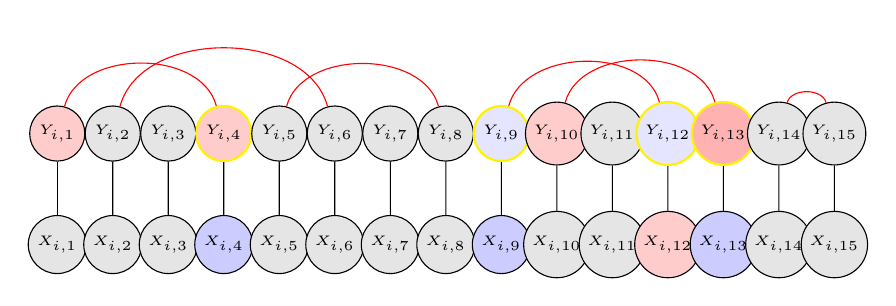
\begin{tikzpicture}[scale=.47]
\tikzstyle{every node} = [draw, shape=circle,minimum size=7mm,inner sep=2pt]
\node [fill = red!20] (a) at (0, 0) {\tiny $Y_{i, 1}$};
\node [fill = gray!20] (b) at (1.5, 0) {\tiny $Y_{i, 2}$};
\node [fill = gray!20](c) at (3, 0) {\tiny $Y_{i, 3}$};
\node [thick, draw = yellow, fill = red!20](d) at (4.5, 0) {\tiny $Y_{i, 4}$};
\node [fill = gray!20](e) at (6, 0) {\tiny $Y_{i, 5}$};
\node [fill = gray!20](f) at (7.5, 0) {\tiny $Y_{i, 6}$};
\node [fill = gray!20] (g) at (9, 0) {\tiny $Y_{i, 7}$};
\node [fill = gray!20](h) at (10.5, 0) {\tiny $Y_{i, 8}$};
\node [thick, draw=yellow,fill = blue!10](i) at (12, 0) {\tiny $Y_{i, 9}$};
\node [fill = red!20](j) at (13.5, 0) {\tiny $Y_{i, 10}$};
\node [fill = gray!20](k) at (15, 0) {\tiny $Y_{i, 11}$};
\node [thick, draw = yellow, fill = blue!10](l) at (16.5, 0) {\tiny $Y_{i, 12}$};
\node [thick, draw = yellow, fill = red!30](m) at (18, 0) {\tiny $Y_{i, 13}$};
\node [fill = gray!20](n) at (19.5, 0) {\tiny $Y_{i, 14}$};
\node [fill = gray!20](o) at (21, 0) {\tiny $Y_{i, 15}$};

\node [fill = gray!20] (ax) at (0, -3) {\tiny $X_{i, 1}$};
\node [fill = gray!20](bx) at (1.5, -3) {\tiny $X_{i, 2}$};
\node [fill = gray!20](cx) at (3, -3) {\tiny $X_{i, 3}$};
\node [fill = blue!20](dx) at (4.5, -3) {\tiny $X_{i, 4}$};
\node [fill = gray!20](ex) at (6, -3) {\tiny $X_{i, 5}$};
\node [fill = gray!20](fx) at (7.5, -3) {\tiny $X_{i, 6}$};
\node [fill = gray!20](gx) at (9, -3) {\tiny $X_{i, 7}$};
\node [fill = gray!20](hx) at (10.5, -3) {\tiny $X_{i, 8}$};
\node [fill = blue!20](ix) at (12, -3) {\tiny $X_{i, 9}$};
\node [fill = gray!20](jx) at (13.5, -3) {\tiny $X_{i, 10}$};
\node [fill = gray!20](kx) at (15, -3) {\tiny $X_{i, 11}$};
\node [fill = red!20](lx) at (16.5, -3) {\tiny $X_{i, 12}$};
\node [fill = blue!20](mx) at (18, -3) {\tiny $X_{i, 13}$};
\node [fill = gray!20](nx) at (19.5, -3) {\tiny $X_{i, 14}$};
\node [fill = gray!20](ox) at (21, -3) {\tiny $X_{i, 15}$};

\draw [-] (ax) to  [out=90,in=270] (a);
\draw [-] (bx) to  [out=90,in=270] (b);
\draw [-] (cx) to  [out=90,in=270] (c);
\draw [-] (dx) to  [out=90,in=270] (d);
\draw [-] (ex) to  [out=90,in=270] (e);
\draw [-] (fx) to  [out=90,in=270] (f);
\draw [-] (gx) to  [out=90,in=270] (g);
\draw [-] (hx) to  [out=90,in=270] (h);
\draw [-] (ix) to  [out=90,in=270] (i);
\draw [-] (jx) to  [out=90,in=270] (j);
\draw [-] (kx) to  [out=90,in=270] (k);
\draw [-] (lx) to  [out=90,in=270] (l);
\draw [-] (mx) to  [out=90,in=270] (m);
\draw [-] (nx) to  [out=90,in=270] (n);
\draw [-] (ox) to  [out=90,in=270] (o);

\draw [-, draw=red] (a) to  [out=75,in=105] (d);
\draw [-, draw=red] (e) to  [out=75,in=105] (h);
\draw [-, draw=red] (b) to  [out=75,in=105] (f);
\draw [-, draw=red] (j) to  [out=75,in=105] (m);
\draw [-, draw=red] (n) to  [out=75,in=105] (o);
\draw [-, draw=red] (i) to  [out=75,in=105] (l);
\end{tikzpicture}
\end{center}
\end{frame}

\begin{frame}
Formula behind the model:
\begin{Definition}
$P(Y|X) = \frac{1}{Z}exp(\alpha\sum\limits_{i}f(y_i,X_i)+\beta\sum\limits_{i,j}g(y_i,y_j))$\\
$f(y_i,X_i) = -(y_i-X_i)^2$,
$g(y_i, y_j, X_i) = -\frac{1}{2}S_{i,j}(y_i-y_j)^2$
\end{Definition}
Previous Example: suppose, we learned small $\alpha$ and large $\beta$. Properties of $Y$ that maximizes $P(Y|X)$:
\begin{itemize}
\item $\beta\sum\limits_{i,j}-\frac{1}{2}S_{i,j}(y_i-y_j)^2$ is idealy close to zero $\Rightarrow$ choose similar predictions for similar targets.
\item $\alpha\sum\limits_{i} -(y_i-X_i)^2$ has little importance $\Rightarrow$ predictions can differ from the MF prediction.
\end{itemize}
\end{frame}

\begin{frame}
\frametitle{Model Evaluation}
Model Evaluation:
\begin{itemize}
\item binary metrics AUC, AUPR $\Rightarrow$ apply threshold to binarize data.
\item Concordance Index (CI): ranking metric.
\end{itemize}
\only<1>{
\begin{center}
{\renewcommand{\arraystretch}{1.2}
\begin{tabular}{c c c}
AUC & AUPR & CI \\
\begin{tabular}{c|c|c} 
2D &  &  \\ \hline
$\delta$ &  & 0.885\\ \hline
 & SW & $\delta$ \\
\end{tabular} & \begin{tabular}{c|c|c} 
2D &  & \\ \hline
$\delta$ & & 0.331\\ \hline
 & SW & $\delta$ \\
\end{tabular} & \begin{tabular}{c|c|c} 
2D &  & \\ \hline
$\delta$ &  & 0.75 \\ \hline
& SW & $\delta$ \\
\end{tabular} 
\end{tabular}}
\end{center}}
\only<2>{
\begin{center}
{\renewcommand{\arraystretch}{1.2}
\begin{tabular}{c c c}
AUC & AUPR & CI \\
\begin{tabular}{c|c|c} 
2D &  &  \\ \hline
$\delta$ & 0.91 & 0.885\\ \hline
 & SW & $\delta$ \\
\end{tabular} & \begin{tabular}{c|c|c} 
2D &  & \\ \hline
$\delta$ &0.431 & 0.331\\ \hline
 & SW & $\delta$ \\
\end{tabular} & \begin{tabular}{c|c|c} 
2D &  & \\ \hline
$\delta$ & 0.77  & 0.75\\ \hline
& SW & $\delta$ \\
\end{tabular} 
\end{tabular}}
\end{center}}
\only<3>{
\begin{center}
{\renewcommand{\arraystretch}{1.2}
\begin{tabular}{c c c}
AUC & AUPR & CI \\
\begin{tabular}{c|c|c} 
2D &  & 0.93 \\ \hline
$\delta$ & 0.91 & 0.885\\ \hline
 & SW & $\delta$ \\
\end{tabular} & \begin{tabular}{c|c|c} 
2D &  & 0.515 \\ \hline
$\delta$ &0.431 & 0.331\\ \hline
 & SW & $\delta$ \\
\end{tabular} & \begin{tabular}{c|c|c} 
2D &  & 0.80\\ \hline
$\delta$ & 0.77  & 0.75\\ \hline
& SW & $\delta$ \\
\end{tabular} 
\end{tabular}}
\end{center}}
\only<4>{
\begin{center}
{\renewcommand{\arraystretch}{1.2}
\begin{tabular}{c c c}
AUC & AUPR & CI \\
\begin{tabular}{c|c|c} 
2D & 0.947 & 0.93 \\ \hline
$\delta$ & 0.91 & 0.885\\ \hline
 & SW & $\delta$ \\
\end{tabular} & \begin{tabular}{c|c|c} 
2D & 0.578 & 0.515 \\ \hline
$\delta$ &0.431 & 0.331\\ \hline
 & SW & $\delta$ \\
\end{tabular} & \begin{tabular}{c|c|c} 
2D & 0.82 & 0.80\\ \hline
$\delta$ & 0.77  & 0.75\\ \hline
& SW & $\delta$ \\
\end{tabular} 
\end{tabular}}
\end{center}}
\end{frame}


\section{Future Work}
\begin{frame}
\frametitle{Causal Inference}
\end{frame}

\begin{frame}
\frametitle{Project Ideas}
\end{frame}

\end{document}